\documentclass[12pt,twoside]{article}

\newcommand{\reporttitle}{Project Interim Report}
\newcommand{\reportauthor}{Dane G. Sherburn}
\newcommand{\reporttype}{Project III}
\newcommand{\cid}{00820119}

% include files that load packages and define macros
%%%%%%%%%%%%%%%%%%%%%%%%%%%%%%%%%%%%%%%%%
% University Assignment Title Page 
% LaTeX Template
% Version 1.0 (27/12/12)
%
% This template has been downloaded from:
% http://www.LaTeXTemplates.com
%
% Original author:
% WikiBooks (http://en.wikibooks.org/wiki/LaTeX/Title_Creation)
%
% License:
% CC BY-NC-SA 3.0 (http://creativecommons.org/licenses/by-nc-sa/3.0/)
% 
% Instructions for using this template:
% This title page is capable of being compiled as is. This is not useful for 
% including it in another document. To do this, you have two options: 
%
% 1) Copy/paste everything between \begin{document} and \end{document} 
% starting at \begin{titlepage} and paste this into another LaTeX file where you 
% want your title page.
% OR
% 2) Remove everything outside the \begin{titlepage} and \end{titlepage} and 
% move this file to the same directory as the LaTeX file you wish to add it to. 
% Then add \input{./title_page_1.tex} to your LaTeX file where you want your
% title page.
%
%----------------------------------------------------------------------------------------
%	PACKAGES AND OTHER DOCUMENT CONFIGURATIONS
%----------------------------------------------------------------------------------------
\usepackage{ifxetex}
\usepackage{textpos}
\usepackage{natbib}
\usepackage{kpfonts}
\usepackage[a4paper,hmargin=2.8cm,vmargin=2.0cm,includeheadfoot]{geometry}
\usepackage{ifxetex}
\usepackage{stackengine}
\usepackage{tabularx,longtable,multirow,subfigure,caption}%hangcaption
\usepackage{fncylab} %formatting of labels
\usepackage{fancyhdr}
\usepackage{color}
\usepackage[tight,ugly]{units}
\usepackage{url}
\usepackage{float}
\usepackage[english]{babel}
\usepackage{amsmath}
\usepackage{graphicx}
\usepackage[colorinlistoftodos]{todonotes}
\usepackage{dsfont}
\usepackage{epstopdf} % automatically replace .eps with .pdf in graphics
\usepackage{natbib}
\usepackage{backref}
\usepackage{array}
\usepackage{latexsym}
\usepackage{etoolbox}

\usepackage{enumerate} % for numbering with [a)] format 



\ifxetex
\usepackage{fontspec}
\setmainfont[Scale=.8]{OpenDyslexic-Regular}
\else
\usepackage[pdftex,pagebackref,hypertexnames=false,colorlinks]{hyperref} % provide links in pdf
\hypersetup{pdftitle={},
  pdfsubject={}, 
  pdfauthor={\reportauthor},
  pdfkeywords={}, 
  pdfstartview=FitH,
  pdfpagemode={UseOutlines},% None, FullScreen, UseOutlines
  bookmarksnumbered=true, bookmarksopen=true, colorlinks,
    citecolor=black,%
    filecolor=black,%
    linkcolor=black,%
    urlcolor=black}
\usepackage[all]{hypcap}
\fi

\usepackage{tcolorbox}

% various theorems
\usepackage{ntheorem}
\theoremstyle{break}
\newtheorem{lemma}{Lemma}
\newtheorem{theorem}{Theorem}
\newtheorem{remark}{Remark}
\newtheorem{definition}{Definition}
\newtheorem{proof}{Proof}

% example-environment
\newenvironment{example}[1][]
{ 
\vspace{4mm}
\noindent\makebox[\linewidth]{\rule{\hsize}{1.5pt}}
\textbf{Example #1}\\
}
{ 
\noindent\newline\makebox[\linewidth]{\rule{\hsize}{1.0pt}}
}



%\renewcommand{\rmdefault}{pplx} % Palatino
% \renewcommand{\rmdefault}{put} % Utopia

\ifxetex
\else
\renewcommand*{\rmdefault}{bch} % Charter
\renewcommand*{\ttdefault}{cmtt} % Computer Modern Typewriter
%\renewcommand*{\rmdefault}{phv} % Helvetica
%\renewcommand*{\rmdefault}{iwona} % Avant Garde
\fi

\setlength{\parindent}{0em}  % indentation of paragraph

\setlength{\headheight}{14.5pt}
\pagestyle{fancy}
\fancyfoot[ER,OL]{\thepage}%Page no. in the left on
                                %odd pages and on right on even pages
\fancyfoot[OC,EC]{\sffamily }
\renewcommand{\headrulewidth}{0.1pt}
\renewcommand{\footrulewidth}{0.1pt}
\captionsetup{margin=10pt,font=small,labelfont=bf}


%--- chapter heading

\def\@makechapterhead#1{%
  \vspace*{10\p@}%
  {\parindent \z@ \raggedright %\sffamily
        %{\Large \MakeUppercase{\@chapapp} \space \thechapter}
        %\\
        %\hrulefill
        %\par\nobreak
        %\vskip 10\p@
    \interlinepenalty\@M
    \Huge \bfseries 
    \thechapter \space\space #1\par\nobreak
    \vskip 30\p@
  }}

%---chapter heading for \chapter*  
\def\@makeschapterhead#1{%
  \vspace*{10\p@}%
  {\parindent \z@ \raggedright
    \sffamily
    \interlinepenalty\@M
    \Huge \bfseries  
    #1\par\nobreak
    \vskip 30\p@
  }}
  



% %%%%%%%%%%%%% boxit
\def\Beginboxit
   {\par
    \vbox\bgroup
	   \hrule
	   \hbox\bgroup
		  \vrule \kern1.2pt %
		  \vbox\bgroup\kern1.2pt
   }

\def\Endboxit{%
			      \kern1.2pt
		       \egroup
		  \kern1.2pt\vrule
		\egroup
	   \hrule
	 \egroup
   }	

\newenvironment{boxit}{\Beginboxit}{\Endboxit}
\newenvironment{boxit*}{\Beginboxit\hbox to\hsize{}}{\Endboxit}



\allowdisplaybreaks

\makeatletter
\newcounter{elimination@steps}
\newcolumntype{R}[1]{>{\raggedleft\arraybackslash$}p{#1}<{$}}
\def\elimination@num@rights{}
\def\elimination@num@variables{}
\def\elimination@col@width{}
\newenvironment{elimination}[4][0]
{
    \setcounter{elimination@steps}{0}
    \def\elimination@num@rights{#1}
    \def\elimination@num@variables{#2}
    \def\elimination@col@width{#3}
    \renewcommand{\arraystretch}{#4}
    \start@align\@ne\st@rredtrue\m@ne
}
{
    \endalign
    \ignorespacesafterend
}
\newcommand{\eliminationstep}[2]
{
    \ifnum\value{elimination@steps}>0\leadsto\quad\fi
    \left[
        \ifnum\elimination@num@rights>0
            \begin{array}
            {@{}*{\elimination@num@variables}{R{\elimination@col@width}}
            |@{}*{\elimination@num@rights}{R{\elimination@col@width}}}
        \else
            \begin{array}
            {@{}*{\elimination@num@variables}{R{\elimination@col@width}}}
        \fi
            #1
        \end{array}
    \right]
    & 
    \begin{array}{l}
        #2
    \end{array}
    &%                                    moved second & here
    \addtocounter{elimination@steps}{1}
}
\makeatother

%% Fast macro for column vectors
\makeatletter  
\def\colvec#1{\expandafter\colvec@i#1,,,,,,,,,\@nil}
\def\colvec@i#1,#2,#3,#4,#5,#6,#7,#8,#9\@nil{% 
  \ifx$#2$ \begin{bmatrix}#1\end{bmatrix} \else
    \ifx$#3$ \begin{bmatrix}#1\\#2\end{bmatrix} \else
      \ifx$#4$ \begin{bmatrix}#1\\#2\\#3\end{bmatrix}\else
        \ifx$#5$ \begin{bmatrix}#1\\#2\\#3\\#4\end{bmatrix}\else
          \ifx$#6$ \begin{bmatrix}#1\\#2\\#3\\#4\\#5\end{bmatrix}\else
            \ifx$#7$ \begin{bmatrix}#1\\#2\\#3\\#4\\#5\\#6\end{bmatrix}\else
              \ifx$#8$ \begin{bmatrix}#1\\#2\\#3\\#4\\#5\\#6\\#7\end{bmatrix}\else
                 \PackageError{Column Vector}{The vector you tried to write is too big, use bmatrix instead}{Try using the bmatrix environment}
              \fi
            \fi
          \fi
        \fi
      \fi
    \fi
  \fi 
}  
\makeatother

\robustify{\colvec}

%%% Local Variables: 
%%% mode: latex
%%% TeX-master: "notes"
%%% End: 
 % various packages needed for maths etc.
% quick way of adding a figure
\newcommand{\fig}[3]{
 \begin{center}
 \scalebox{#3}{\includegraphics[#2]{#1}}
 \end{center}
}

%\newcommand*{\point}[1]{\vec{\mkern0mu#1}}
\newcommand{\ci}[0]{\perp\!\!\!\!\!\perp} % conditional independence
\newcommand{\point}[1]{{#1}} % points 
\renewcommand{\vec}[1]{{\boldsymbol{{#1}}}} % vector
\newcommand{\mat}[1]{{\boldsymbol{{#1}}}} % matrix
\newcommand{\R}[0]{\mathds{R}} % real numbers
\newcommand{\Z}[0]{\mathds{Z}} % integers
\newcommand{\N}[0]{\mathds{N}} % natural numbers
\newcommand{\nat}[0]{\mathds{N}} % natural numbers
\newcommand{\Q}[0]{\mathds{Q}} % rational numbers
\ifxetex
\newcommand{\C}[0]{\mathds{C}} % complex numbers
\else
\newcommand{\C}[0]{\mathds{C}} % complex numbers
\fi
\newcommand{\tr}[0]{\text{tr}} % trace
\renewcommand{\d}[0]{\mathrm{d}} % total derivative
\newcommand{\inv}{^{-1}} % inverse
\newcommand{\id}{\mathrm{id}} % identity mapping
\renewcommand{\dim}{\mathrm{dim}} % dimension
\newcommand{\rank}[0]{\mathrm{rk}} % rank
\newcommand{\determ}[1]{\mathrm{det}(#1)} % determinant
\newcommand{\scp}[2]{\langle #1 , #2 \rangle}
\newcommand{\kernel}[0]{\mathrm{ker}} % kernel/nullspace
\newcommand{\img}[0]{\mathrm{Im}} % image
\newcommand{\idx}[1]{{(#1)}}
\DeclareMathOperator*{\diag}{diag}
\newcommand{\E}{\mathds{E}} % expectation
\newcommand{\var}{\mathds{V}} % variance
\newcommand{\gauss}[2]{\mathcal{N}\big(#1,\,#2\big)} % gaussian distribution N(.,.)
\newcommand{\gaussx}[3]{\mathcal{N}\big(#1\,|\,#2,\,#3\big)} % gaussian distribution N(.|.,.)
\newcommand{\gaussBig}[2]{\mathcal{N}\left(#1,\,#2\right)} % see above, but with brackets that adjust to the height of the arguments
\newcommand{\gaussxBig}[3]{\mathcal{N}\left(#1\,|\,#2,\,#3\right)} % see above, but with brackets that adjust to the height of the arguments
\DeclareMathOperator{\cov}{Cov} % covariance (matrix) 
\ifxetex
\renewcommand{\T}[0]{^\top} % transpose
\else
\newcommand{\T}[0]{^\top}
\fi
% matrix determinant
\newcommand{\matdet}[1]{
\left|
\begin{matrix}
#1
\end{matrix}
\right|
}



%%% various color definitions
\definecolor{darkgreen}{rgb}{0,0.6,0}

\newcommand{\blue}[1]{{\color{blue}#1}}
\newcommand{\red}[1]{{\color{red}#1}}
\newcommand{\green}[1]{{\color{darkgreen}#1}}
\newcommand{\orange}[1]{{\color{orange}#1}}
\newcommand{\magenta}[1]{{\color{magenta}#1}}
\newcommand{\cyan}[1]{{\color{cyan}#1}}


% redefine emph
\renewcommand{\emph}[1]{\blue{\bf{#1}}}

% place a colored box around a character
\gdef\colchar#1#2{%
  \tikz[baseline]{%
  \node[anchor=base,inner sep=2pt,outer sep=0pt,fill = #2!20] {#1};
    }%
}%
 % short-hand notation and macros

% for minimalistic tables
\usepackage{booktabs}

% for plotting subfigures
%\usepackage[demo]{graphicx}
%\usepackage{subcaption}%  http://ctan.org/pkg/subcaption   
\captionsetup[subfigure]{labelformat = parens, labelsep = space, font = small}


%%%%%%%%%%%%%%%%%%%%%%%%%%%%

\begin{document}

% front page
% Last modification: 2016-09-29 (Marc Deisenroth)
\begin{titlepage}

\newcommand{\HRule}{\rule{\linewidth}{0.5mm}} % Defines a new command for the horizontal lines, change thickness here


%----------------------------------------------------------------------------------------
%	LOGO SECTION
%----------------------------------------------------------------------------------------


\includegraphics[width = 4cm]{./figures/imperial}\\[0.5cm] 

\begin{center} % Center remainder of the page

%----------------------------------------------------------------------------------------
%	HEADING SECTIONS
%----------------------------------------------------------------------------------------
\vspace{1.5cm}
\textsc{\Large Imperial College London}\\[0.5cm]
\textsc{\large Department of Computing}\\[0.5cm] 
%----------------------------------------------------------------------------------------
%	TITLE SECTION
%----------------------------------------------------------------------------------------

\HRule \\[0.4cm]
{ \huge \bfseries \reporttitle}\\ % Title of your document
\HRule \\[1.5cm]
\end{center}
%----------------------------------------------------------------------------------------
%	AUTHOR SECTION
%----------------------------------------------------------------------------------------

%\begin{minipage}{0.4\hsize}
\begin{flushleft} \large
\textit{Author:}\\
\reportauthor~\\
\vspace{1cm}
\textit{CID:}\\
\cid % Your name
\end{flushleft}
\vspace{2cm}
\makeatletter
Date: \@date 

\vfill % Fill the rest of the page with whitespace



\makeatother


\end{titlepage}


\newpage

% table of contents
\tableofcontents
\newpage

% bibliography style
\bibliographystyle{unsrt} 

%%%%%%%%%%%%%%%%%%%%%%%%%%%% Main document
\section{Introduction}
A long term goal of artificial intelligence (AI) is the development of artificial general intelligence (AGI). A number of theoretical frameworks have been presented to formalize what it means to achieve AGI, notably by Hutter \cite{Hutter2005}.\\

Reinforcement learning is fundamental in this framework. It's therefore quite exciting that deep reinforcement learning (DRL) systems have recently been able to master a wide range of tasks, including Atari games and Go. Though DRL systems have been remarkably successful, they still have a number of drawbacks \cite{Garnelo2016}:

\begin{enumerate}
\item \textbf{Slow to learn}. Deep neural networks require large data sets and are therefore slow to learn.
\item \textbf{Fail to transfer past experience}. They often fail to perform well on tasks very similar to those they have mastered.
\item \textbf{Inability to reason abstractly.} They fail to exploit statistical regularities in the training data by using high-level processes like planning or causal reasoning.
\item \textbf{Hard to reason about.} It's often troublesome to understand why the DRL system chose the action it did.
\end{enumerate}

Deep symbolic reinforcement learning (DSRL) is a recent advance which overcomes all of these drawbacks at once without the drawbacks from classical symbolic AI, namely the symbol grounding problem \cite{Garnelo2016}.\\

This novel architecture relies on the unsupervised extraction of compositional features, allowing for transfer learning and high-level cognitive processes. However, the unsupervised extraction of features from a wide range of scenes is still a challenge in AI research \cite{Bengio2013}. Fortunately methods are getting better, and the first unsupervised scalable model $\beta$-VAE was developed recently. \\

The aim of this project is to investigate compositional representations using $\beta$-VAE and evaluate their effectiveness in deep symbolic reinforcement systems. We plan to achieve this as follows:

\begin{enumerate}
\item Implement many flavours of autoencoders, including mixing and matchings of standard, convolutional and variational autoencoders, and investigate the relationship between the latent space and their final reconstructions. This will hopefully convey some intuition about the way scenes are typically represented in the latent space, their relevance in transfer learning and the significance of the problem we're trying to solve.
\item Next we focus our attention on convolutional variational autoencoders. We'll experiment with different values of $\beta$ two ways: through heuristic visual inspection, and by comparing the disentanglement metric and reconstruction error. All experiments will be on a range of Atari 2600 games using the Atari Learning Environment.
\item Finally we can evaluate the value of a compositional structured latent space in a deep symbolic reinforcement system. We'll do this by training a number of reinforcement agents on the latent space and compare their performance to training on the on the original space. We can also train the one agent on multiple games to assess how well this compositional structure facilitates transfer learning.
\end{enumerate}

\section{Background}
This chapter will contain the material necessary to understand later chapters and provide the context for our contributions.\\

We will introduce deep symbolic reinforcement learning which will motivate our interest in unsupervised disentangled representations. Here we'll explore state-of-the-art approaches to finding such representations, which will also require a brief introduction to autoencoders. Finally we'll mention less theoretical matters, including libraries used and the Arcade Learning Environment.

% Autoencoders
\subsection{Autoencoders}

\subsubsection{Architecture}

Autoencoders are standard feed-forward networks with a ``bottleneck" in a hidden layer, shown in Figure (\ref{fig:autoencoder_encoder_decoder}). Autoencoders learn the identity function $f(\vec{x})=\vec{x}$, which may seem pointless at first. However, if the autoencoder closely approximates the identity function, the decoder is actually computing a reconstruction of the original image $\widetilde{\vec{x}}$ from a lower-dimensional representation $\vec{z}$, called the \textit{latent space}. So for any given $\vec{x}$, we can compute a compressed version, $\vec{z}$, by submitting $\vec{x}$ to the encoder. This compression technique is data-specific and, at present, isn't scalable \cite{Chollet2016}. However, they are very effective at denoising images and likely to play an important role in reverse Google image searches \cite{Krizhevsky2011}.\\

The type of feed-forward network chosen depends on the nature of the data. We'll be using images as our input data, so the natural choice is to use convolutional neural networks. Our encoder will include convolutional and pooling layers to learn relevant features and downsample the data respectively, and our decoder will include deconvolutional and upsampling layers (as they're natural inverses).

\begin{figure}
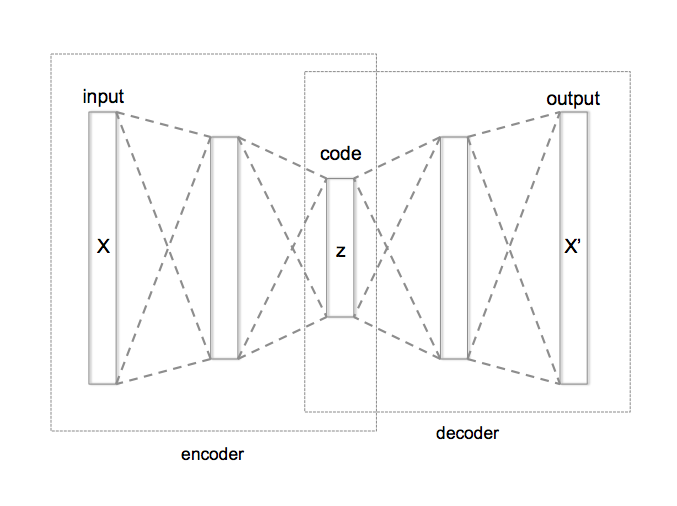
\includegraphics[scale=0.5]{figures/autoencoder_encoder_decoder.png}
\centering
\captionsetup{justification=centering}
\caption{Autoencoders can be split into the encoder, which takes input $\vec{x}$ and outputs the low-dimensional $\vec{z}$, and the decoder, which takes input $\vec{z}$ and tries to reconstruct $\vec{x}$.}
\label{fig:autoencoder_encoder_decoder}
\end{figure}

\begin{figure}
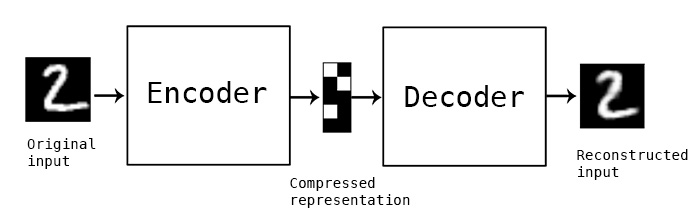
\includegraphics[scale=2.0]{figures/autoencoder_black_box.jpg}
\centering
\captionsetup{justification=centering}
\caption{A black-box view of the autoencoder showing the relationship between the encoder and decoder. The latent space shown in the center is clearly of a lower dimension than the input, acting as a code. \cite{Chollet2016}}
\label{fig:autoencoder_black_box}
\end{figure}

\subsubsection{Convolutional autoencoders}

\subsubsection{Variational autoencoders}

The autoencoders we've seen so far do the following: given input $\vec{x}$, compute its reconstruction $\widetilde{\vec{x}}$, after mapping it to a lower dimensional vector $\vec{z}$, the \textit{latent space}. The aim of the variational autoencoder (VAE) is quite similar: given input samples from an unknown distribution $p(\vec{x})$, generate $\widetilde{\vec{x}}$ very similar to those in $p(\vec{x})$, after sampling a lower-dimensional vector $\vec{z}$. Since VAEs generate unseen, similar samples, they are \textit{generative models} \cite{Doersch2016}.\\

To justify the statements in the next paragraph, we have to mention that $p_{\theta}(\vec{z}|\vec{x})=\frac{p(\vec{x}|\vec{z})p(\vec{z})}{p(\vec{x})}$ is intractable due to the marginal likelihood $p(\vec{x})$ being exponentially computationally expensive, motivating the introduction of the probabilistic encoder $q_{\phi}(\vec{z}|\vec{x})$ to approximate the posterior $p_{\theta}(\vec{z}|\vec{x})$. Since $q_{\phi}(\vec{z}|\vec{x})$ appears in the loss function but is not differentiable (we can't differentiate random variables), we need to use the \textit{reparameterisation trick}. The reparameterisation trick expresses $\vec{z}\sim q_{\phi}(\vec{z}|\vec{x})$ as a deterministic variable $\vec{z}=g_{\phi}(\vec{\epsilon},\vec{x})$ where $\vec{\epsilon}$ is an auxilary variable with independent maginal and $g_{\phi}$ is a deterministic vector function parameterized by $\phi$ \cite{Kingma2014}.\\

Learning the optimal $\vec{\phi}$ and $\vec{\theta}$ is formally expressed as the following objective:
\begin{equation}
\label{vae_objective}
\max_{\vec{\phi},\vec{\theta}}\mathbf{E}_{q_{\phi}(\vec{z}|\vec{x})}[log p_{\theta}(\vec{x}|\vec{z})] - \mathcal{D}_{KL}[q_{\phi}(\vec{z}|\vec{x})||p_{\theta}(\vec{z})]
\end{equation}


% Deep symbolic reinforcement learning
\subsection{Deep symbolic reinforcement learning}

\subsubsection{Reinforcement learning}

\subsubsection{Symbolic artificial intelligence}

\subsubsection{Deep symbolic reinforcement learning}

% Representation learning
\subsection{Representation learning}

Suppose we were ordered to carry out the multiplication of two binary numbers, $1101_2$ and $101101_2$. Most of us would first convert these numbers to base-10 before performing the multiplication. We'd do this because the problem is significantly harder in base-2 than it is in base-10. It's therefore intuitive that a good representation is vital to the agent required to solve it \cite{IanGoodfellowYoshuaBengio2015}.\\

The subject of what makes a good representation has generated much interest in recent times. According to \cite{IanGoodfellowYoshuaBengio2015}, a good representation is simply one that makes subsequent tasks easier. 

\subsubsection{Disentangled representations}

It's been suggested by \cite{Bengio2013} that a crucial factor in what makes a good representation is how \textit{disentangled} it is. A disentangled representation is one where changes in latent factors correspond to changes in high-level factors in the output space \cite{Higgins2016}.\\

To provide some intuition of what a disentangled representation is, we'll consider an example using the Frey Face data set.\\

\begin{figure}
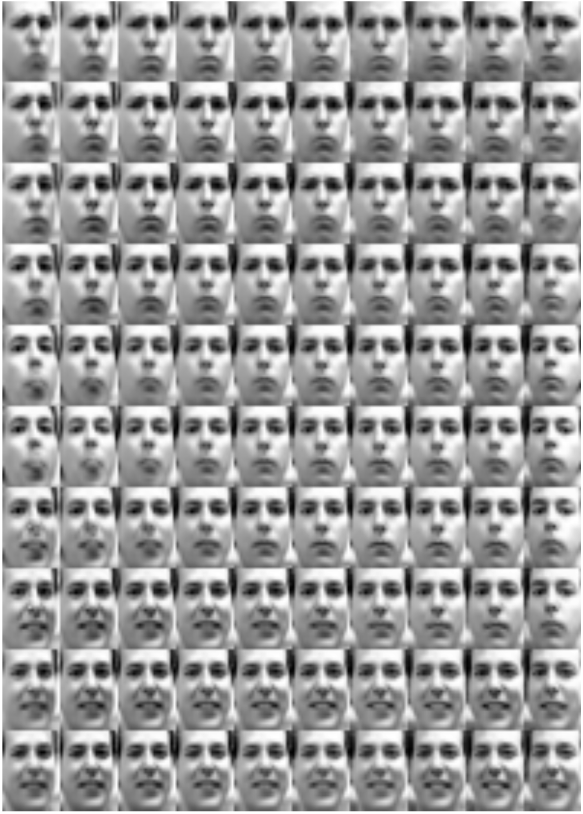
\includegraphics[scale=0.3]{figures/kingma_2014_4a.png}
\centering
\captionsetup{justification=centering}
\caption{A learned Frey Face manifold with two latent variables: one sensitive to the expression and one to the orientation. \cite{Kingma2014}}
\label{frey_face_disentangled}
\end{figure}

The Frey Face data set consists of almost two-thousand $28\times20$ pictures of Brendan Frey, a Canadian machine learning researcher. The samples include Frey with varying facial expressions and orientations.\\

Shown in Figure (\ref{frey_face_disentangled}) is a learned Frey Face manifold with two latent variables. One latent variable is sensitive to changes in the expression and one to changes in orientation, making the manifold a highly disentangled representation. In an entangled representation, changing one latent variable would change both the expression and the orientation.\\

Disentangled representations facilitate the reuse of previously learnt factors, called \textit{knowledge transfer}; and the extreme case, \textit{zero-shot inference} \cite{IanGoodfellowYoshuaBengio2015,Higgins2016}.

\subsubsection{Transfer learning}
\label{subsec:transfer_learning}
Transfer learning is the reuse of learnt factors from a previous task when learning a new one \cite{IanGoodfellowYoshuaBengio2015}. If the tasks are sufficiently similar, there are three ways the learning may be improved \cite{Torrey2009}:

\begin{enumerate}
\item Initial performance
\item Faster to learn
\item Final performance
\end{enumerate}

These improvements are shown on a performance-training graph in Figure \ref{transfer_learning_three_ways}.\\

\begin{figure}
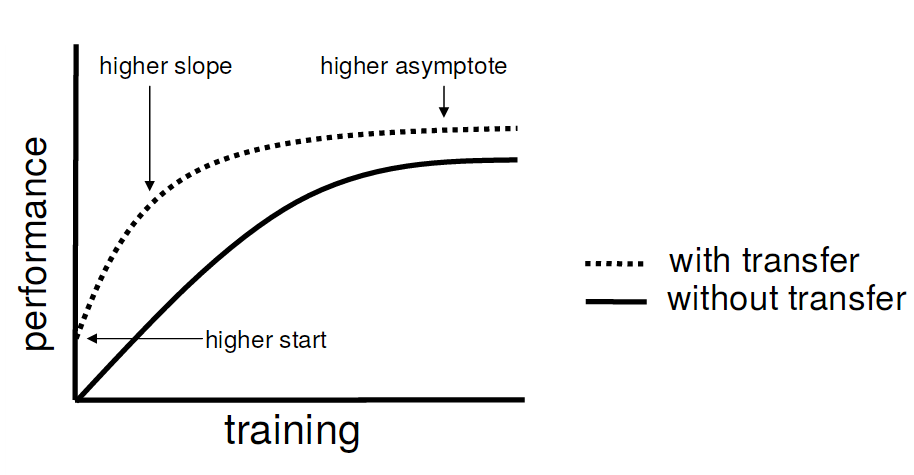
\includegraphics[scale=0.3]{figures/torrey_2009_2.png}
\centering
\captionsetup{justification=centering}
\caption{An illustration of the three ways in which transfer learning may improve the learning of a new task. \cite{Torrey2009}}
\label{transfer_learning_three_ways}
\end{figure}

\begin{figure}
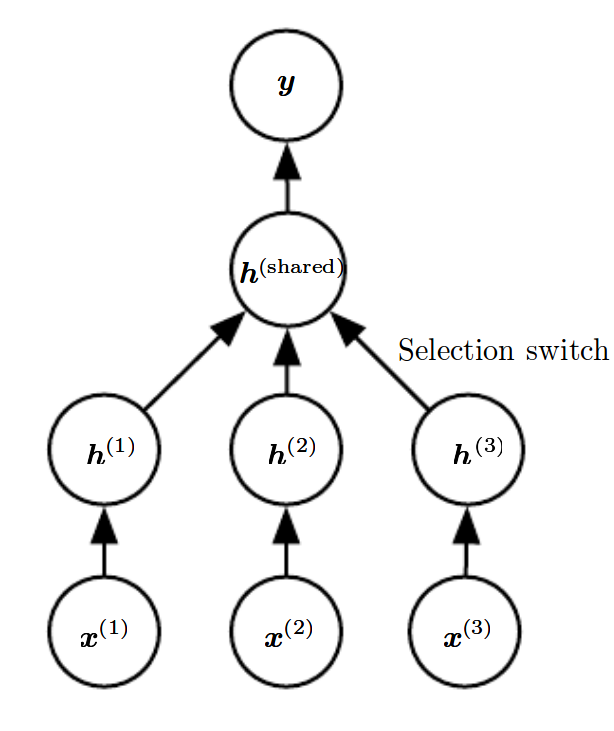
\includegraphics[scale=0.3]{figures/goodfellow_2015_15_2.png}
\centering
\captionsetup{justification=centering}
\caption{An illustration of how tasks may be translated into intermediate representations, then into a shared representation. The representation of different tasks in terms of common concepts is key to transfer learning. \cite{IanGoodfellowYoshuaBengio2015}}
\label{transfer_learning_graph_intuition}
\end{figure}

Entangled representations make it difficult to learn common generative factors among different tasks, as no one latent factor has meaning itself \cite{Whitney2016}.

\subsubsection{Zero-shot understanding}

% Deeper investigation of $\beta$-VAE
\subsection{Deeper investigation of $\beta$-VAE}
\subsubsection{Framework}

Suppose we're given a set $X$ of images $\vec{x}\in\mathbb{R}^N$ and ground truth data generative factors (that is, factors observed directly from the data as opposed to being inferred). We'll partition these factors into two sets, $V$ and $W$, where vectors $\vec{v}\in\mathbb{R}^K$ are independent and $\vec{w}\in\mathbb{R}^H$ are dependent.\\

The aim of $\beta$-VAE is to factorise the latent space $\vec{z}\in\mathbb{R}^M$ into disentangled factors $\vec{v}$ and the rest. This enforces $M\geq K$, since we'd like the latent representation to be capable of learning all independent ground truth data factors of $X$.\\

$\beta$-VAE achieves this by adding an important multiplicative factor $\beta$ to the KL-divergence term, making the objective:

\begin{equation}
\label{beta_vae_objective}
\max_{\vec{\phi},\vec{\theta}}\mathbf{E}_{q_{\phi}(\vec{z}|\vec{x})}[log p_{\theta}(\vec{x}|\vec{z})] - \beta\mathcal{D}_{KL}[q_{\phi}(\vec{z}|\vec{x})||p_{\theta}(\vec{z})]
\end{equation}

The hyperparameter $\beta$ balances reconstruction error with independence constraints \cite{Higgins2016}.

\subsubsection{Disentanglement metric}
\subsubsection{Quantitative performance}
\subsubsection{Qualitative performance}

% Libraries
\subsection{Libraries}
\subsubsection{Keras}

Keras is a high-level neural network library written in Python \cite{Chollet2015} and was used to implement the frameworks in Chapter X. It was a suitable choice because it supports:

\begin{itemize}
\item Convolutional, deconvolutional and pooling layers
\item Lambda functions, which is necessary for sampling in variational autoencoders
\item Custom loss functions, which is necessary to implement the $\beta$-VAE framework
\item Able to save weights, so the same network can be trained on multiple games
\item Able to run on the GPU
\end{itemize}

\subsubsection{Arcade Learning Environment}
The Arcade Learning Environment (ALE) is a framework built on top of the Atari 2600 emulator Stella \cite{Bellemare2015}. This library was a suitable choice because:
\begin{itemize}
\item Emulation details are abstracted away from the researcher
\item The same agent can be used for all games, due to its modular design
\item Frames can be saved during game play, which is used to collect training data
\item A Python wrapper for the entire framework is provided, so our agents developed in Keras interact seamlessly
\end{itemize}

\section{Results}
\label{sec:results}

The ALE was used to capture frames from the emulator Stella at regular intervals, which were dumped into a common location, forming the training set. A convolutional variational autoencoder was then implemented in Keras to train on this data. A number of scripts (that partition the data into training, validation and test sets, for instance) were used in creating generic data sets that are easily loaded into Keras.\\

The VAE was used to generate new samples from the test set using a sample input, shown in Figure (\ref{fig:space_invaders_original}). The sampled latent space and its reconstruction are shown in Figure (\ref{tab:latent_vs_reconstruction_grid}) for different epochs. As expected, the reconstruction improves with the number of epochs.\\

Interestingly, the VAE has already learnt that the upper triangler section of the enemies is more dense than the lower half. It also has picked up on persistent objects, like the three barriers in the center and the floor.

\begin{figure}[h!]
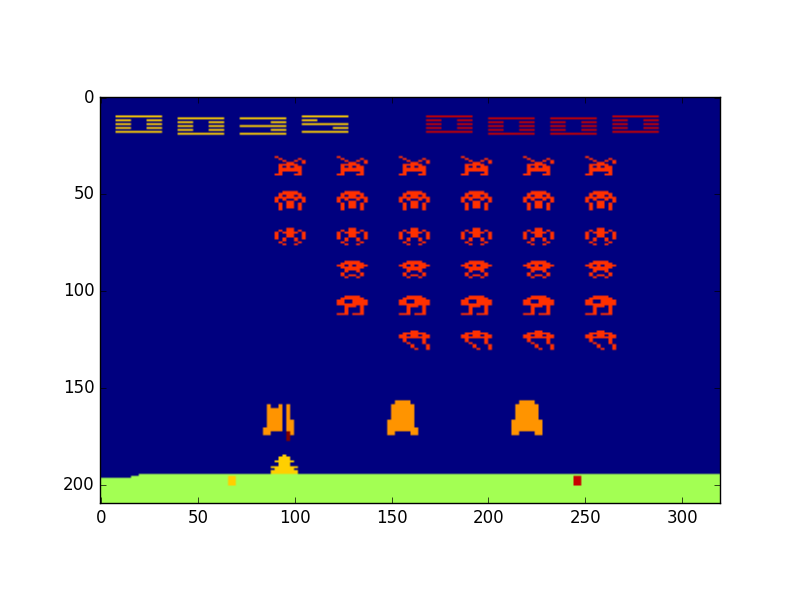
\includegraphics[scale=0.6]{figures/space_invaders_original.png}
\centering
\caption{A screenshot from Space Invaders running in the ALE.}
\label{fig:space_invaders_original}
\end{figure}

\newcommand\cincludegraphics[2][]{\raisebox{-0.3\height}{\includegraphics[#1]{#2}}}
\begin{table}[]
\centering
\captionsetup{justification=centering}
\caption{The latent space and reconstruction for $10$, $50$ and $100$ epochs given Figure (\ref{fig:space_invaders_original}) as input.}
\label{tab:latent_vs_reconstruction_grid}
\begin{tabular}{lll}
\toprule
\hspace{0.8cm} Latent space & \hspace{1cm} Reconstruction \\ \midrule
\cincludegraphics[height=1.7in]{figures/latent_space_latent_16_epochs_10.pdf} & \cincludegraphics[height=2.5in]{figures/reconstruction_latent_16_epochs_10.pdf} &  \\
\cincludegraphics[height=1.7in]{figures/latent_space_latent_16_epochs_50.pdf} & \cincludegraphics[height=2.5in]{figures/reconstruction_latent_16_epochs_50.pdf} &  \\
\cincludegraphics[height=1.7in]{figures/latent_space_latent_16_epochs_100.pdf} & \cincludegraphics[height=2.5in]{figures/reconstruction_latent_16_epochs_100.pdf} &  \\
\end{tabular}
\end{table}


\newpage
\section{Project Plan}
The rough plan for the project is given in Table (\ref{tab:project_plan}). Since the method we will use to evaluate the disentangled representations is still in development, it's not yet possible to assign specific tasks for its implementation. However, the key milestones not dependent on the evaluation have been included as a skeleton to build on in the coming months.\\

% uses \usepackage{booktabs}
\newcommand{\tabitem}{~~\llap{\textbullet}~~}
\begin{table}[h!]
\centering
\caption{Project plan in terms of remaining months.}
\label{tab:project_plan}
\begin{tabular}{@{}lll@{}}
\toprule
                  & \textbf{Milestones}                 & \textbf{Fallbacks}             \\ \midrule
\textbf{February} & \tabitem Implement $\beta$-VAE      & \tabitem Implement $\beta$-VAE \\
                  & \tabitem Reproduce results from \cite{Higgins2016} & \tabitem Reproduce results from \cite{Higgins2016}\\
                  & \tabitem Finish formal justification of VAE &  \\
\textbf{March}    & \tabitem Disentanglement metric script & \tabitem Disentanglement metric script \\
                  & \tabitem Test script with simple data & \tabitem Test script with simple data   \\
\textbf{April}    & \tabitem Find suitable $\beta$ for Pong & \tabitem Find suitable $\beta$ for Pong \\
                  & \tabitem Find suitable $\beta$ for Space Invaders & \tabitem Find suitable $\beta$ for Space Invaders \\
                  & \tabitem Graph latent vs output &                    \\                  
\textbf{May}      & \tabitem Complete report background & \\
                  & \tabitem Complete report related work &                    \\                  
\textbf{June}     & \tabitem Complete report results      &                    \\ \bottomrule
\end{tabular}
\end{table}

The achievements to date are covered in Chapter \ref{sec:results}, and the milestones set out for (at least the immediate months) are a feasible goals. If we are ahead of schedule, the following extensions would be interesting to explore:

\begin{itemize}
\item Train an agent on multiple similar games (Pong and Space Invaders, for instance) to demonstrate the ability of a disentangled representation to facilitate transfer learning, as listed in Subsection \ref{subsec:transfer_learning}.
\item A \textit{generative adversarial network} could be used as the anomoly detection network (described in Chapter \ref{sec:evaluation_plan}), instead of a regular feed-forward network.
\item We could investigate the way the variational autoencoder explores its statespace. To explore its statespace, the autoencoder can endlessly recombine combinations of disentangled factors to produce new samples that may or may not occur in the real worl. For instance, we know not all things that are red and yellow are strawberries and bananas. We can therefore pry apart these two generative factors into a colour and an object. We can then imagine a red banana and a yellow strawberry even though we've never seen either before.
\item Using the previous concept, we could experiment with the agent performing offline-exploration or ``look ahead" in an Atari game.
\item Try using 3D convolutions in encoder and decoder to see how temporal information could be encoded \cite{Ji2013}. It may also be worthwhile to see if this improves any elements in reconstruction error or learning rate. 
\end{itemize}



\newpage
\section{Evaluation plan}
\label{sec:evaluation_plan}
There are two ways in which the representations found may be evaluated: how realistic the generations seem and the degree in which the latent space is disentangled.\\

The decoded images from the sampled disentangled latent space should be as realistic as possible. However the task of visually examining multiple decoded images from multiple alternative latent spaces is time consuming. To automate this process, we could implement an anomoly detection network, which is trained on the whole space of input images. This can be used in the following procedure: train a VAE for a given $\beta$, then generate unseen samples from the dataset and run each through the anomoly detection network. The more images that pass, the higher the score. Performing exponential search on $\beta>1$ would find a suitable disentangled representation without the need for time-consuming visual inspection.\\

As well as using the disentanglement metric introduced in \cite{Higgins2016}, we may quantify how disentangled the latent space is by the following procedure: create an artificial data set varying one generative factor (the paddle in Pong, for instance), and measure the change in latent variables for each of these as inputs. We'd expect a perfectly disentangled latent space to have exactly one latent variable changing value, and remain constant for other data sets changing other generative factors (the ball in Pong, for instance). The changes may be averaged over the number of inputs to give a final disentanglement score.\\

The project would be a success if a suitable range of values of $\beta$ were found such that the generative features in multiple Atari agents were captured, and the benefits of this representation were demonstraed by an agent being able to re-use the same concept in a range of games.

\newpage
\bibliography{library}

\end{document}